\documentclass[a4paper,12pt]{extarticle}
\usepackage[utf8x]{inputenc}
\usepackage[T1,T2A]{fontenc}
\usepackage[russian]{babel}
\usepackage{hyperref}
\usepackage{indentfirst}
\usepackage{listings}
\usepackage{color}
\usepackage{here}
\usepackage{array}
\usepackage{multirow}
\usepackage{graphicx}
\usepackage{algorithm}
\usepackage{algpseudocode}
\usepackage{caption}
\usepackage{pdfpages}
\usepackage{tikz,mathpazo}
\usepackage{graphicx,amssymb,amstext,amsmath,newtxmath}
\usetikzlibrary{shapes.geometric, arrows}
\renewcommand{\lstlistingname}{Программа} % заголовок листингов кода

\bibliographystyle{ugost2008ls}

\usepackage{listings}
\lstset{ %
extendedchars=\true,
keepspaces=true,
language=C,						% choose the language of the code
basicstyle=\footnotesize,		% the size of the fonts that are used for the code
numbers=left,					% where to put the line-numbers
numberstyle=\footnotesize,		% the size of the fonts that are used for the line-numbers
stepnumber=1,					% the step between two line-numbers. If it is 1 each line will be numbered
numbersep=5pt,					% how far the line-numbers are from the code
backgroundcolor=\color{white},	% choose the background color. You must add \usepackage{color}
showspaces=false				% show spaces adding particular underscores
showstringspaces=false,			% underline spaces within strings
showtabs=false,					% show tabs within strings adding particular underscores
frame=single,           		% adds a frame around the code
tabsize=2,						% sets default tabsize to 2 spaces
captionpos=t,					% sets the caption-position to top
breaklines=true,				% sets automatic line breaking
breakatwhitespace=false,		% sets if automatic breaks should only happen at whitespace
escapeinside={\%*}{*)},			% if you want to add a comment within your code
postbreak=\raisebox{0ex}[0ex][0ex]{\ensuremath{\color{red}\hookrightarrow\space}},
texcl=true,
inputpath=listings,                     % директория с листингами
}

\usepackage[left=2cm,right=2cm,
top=2cm,bottom=2cm,bindingoffset=0cm]{geometry}

%% Нумерация картинок по секциям
\usepackage{chngcntr}
\counterwithin{figure}{section}
\counterwithin{table}{section}

%%Точки нумерации заголовков
\usepackage{titlesec}
\titlelabel{\thetitle.\quad}
\usepackage[dotinlabels]{titletoc}

%% Оформления подписи рисунка
\addto\captionsrussian{\renewcommand{\figurename}{Рисунок}}
\captionsetup[figure]{labelsep = period}

%% Подпись таблицы
\DeclareCaptionFormat{hfillstart}{\hfill#1#2#3\par}
\captionsetup[table]{format=hfillstart,labelsep=newline,justification=centering,skip=-10pt,textfont=bf}

%% Путь к каталогу с рисунками
\graphicspath{{fig/}}

%% Внесение titlepage в учёт счётчика страниц
\makeatletter
\renewenvironment{titlepage} {
 \thispagestyle{empty}
}
\makeatother


\begin{document}	% начало документа

% Титульная страница
\begin{titlepage}	% начало титульной страницы

	\begin{center}		% выравнивание по центру

		\large Санкт-Петербургский политехнический университет Петра Великого\\
		\large Физико-механический институт \\
		\large Высшая школа прикладной математики и вычислительной физики\\[3cm]
		% название института, затем отступ 6см
		\large Направление подготовки\\
		\large "01.03.02. Прикладная математика и информатика"\\[3cm]
		\huge Дисциплина "Численные методы"\\[0.5cm] % название работы, затем отступ 0,5см
		\large Отчет по лабораторной работе №3\\[0.1cm]
		\large "Решение СЛАУ итерационными методами. Метод простых итераций"\\[5cm]

	\end{center}


	\begin{flushright} % выравнивание по правому краю
		\begin{minipage}{0.25\textwidth} % врезка в половину ширины текста
			\begin{flushleft} % выровнять её содержимое по левому краю

				\large\textbf{Работу выполнил:}\\
				\large Иванова А.С.\\
				\large {Группа:} 5030102/00002\\
				
				\large \textbf{Преподаватель:}\\
				\large Курц В.В.

			\end{flushleft}
		\end{minipage}
	\end{flushright}
	
	\vfill % заполнить всё доступное ниже пространство

	\begin{center}
	\large Санкт-Петербург\\
	\large \the\year % вывести дату
	\end{center} % закончить выравнивание по центру

\end{titlepage} % конец титульной страницы

\vfill % заполнить всё доступное ниже пространство


% Содержание
\renewcommand\contentsname{\centerline{Содержание}}
\tableofcontents
\newpage



\section{Формулировка задачи}

Дана функция 
\begin{math} 
	y=\sqrt{\sin{x^{2}}}
\end{math}

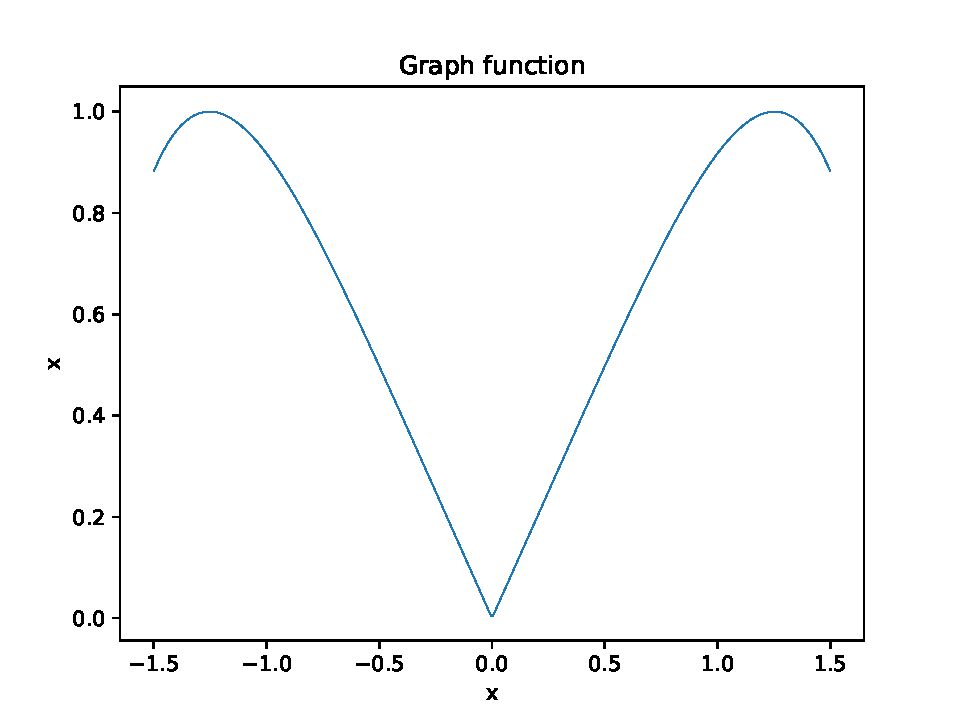
\includegraphics[scale=0.75]{func.pdf}

Требуется вычислить определенный интеграл заданной функции на нескольких отрезках квадратурными формулами интерполяционного типа (в данном случае формула Симпсона). Исследовать влияние заданной точности на объем вычислений, влияние гладкости функций на точность вычислений.

\section{Алгоритм метода и условия его применимости}

\subsection{Алгоритм метода}

Дана функция, которую нужно интегрировать на отрезке [a;b] и количество интервалов, на которое разбивается отрезок N. 

Рассмотрим квадратурные формулы. Представим определенный интеграл на промежутке [a;b] функции F(x) в виде:


Пусть 

\begin{math} 
	\int\limits_{a}^{b}F(x)dx=\int\limits_{a}^{b}p(x)f(x)dx
\end{math}

Формулы вида:

\begin{math} 
	\\
	\int\limits_{a}^{b}p(x)f(x)dx=\sum\limits_{k=1}^{N}A_{k}f(x_{k})dx \\
	A_{k} , x_{k}
\end{math}
- коэффициенты и узлы квадратурной формулы. 

Рассмотрим квадратурные формулы интерполяционного типа: 

Строим табличную функцию на данном нам участке и строим на данной табличной функции интерполяционный полином Лагранжа.

\begin{math} 
	\\
	A_{k}=\int\limits_{a}^{b}p(x)\phi_{k}(x)dx \\
	\phi_{k}(x)=\prod\limits_{j=1,j\neq k}^{N}\frac{x-x_{j}}{x_{k}-x_{j}}
\end{math}

Для того чтобы квадратурная формула имела алгебраический порядок точности n−1 или выше, необходимо и достаточно, чтобы она была интерполяционной.

Квадратурные формулы Ньютона-Котеса - это интерполяционные квадратурные формулы, для которых выполнены следующие условия: 

\begin{math} 
	\\
	1. p(x)=1 \\
	2. x_{k}=a+h(k-1); h=\frac{b-a}{N-1} \\
		\\
	A_{k}=\int\limits_{a}^{b}p(x)\phi_{k}(x)dx \\
	\phi_{k}(x)=\prod\limits_{j=1,j\neq k}^{N}\frac{x-x_{j}}{x_{k}-x_{j}}
\end{math}

Если степень интерполяционного полинома равна 3, то мы получаем формулу Симпсона, имеющую гарантированный алгебраический порядок точности 3. 

\begin{math} 
	h=\frac{b-a}{2N}; x_{k}=a+h*k, k=0,...,N
\end{math}

Формула для одного учаcтка [a;b]
\begin{math} 
	\int\limits_{a}^{b}f(x)dx=\frac{b-a}{6}*(f(a)+4*f(\frac{a+b}{2})+f(b))
\end{math}


Интеграл будет вычисляться как сумма интегралов на разбиениях промежутка (метод Котеса) по следующей формуле:

\begin{math} 
	\int\limits_{a}^{b}f(x)dx=\frac{h}{3}(f(x_{0})+4\sum\limits_{i=1}^{N}f(x_{2i-1})+2\sum\limits_{i=1}^{N-1}f(x_{2i})+f(x_{2N}))
\end{math}

Для оценки погрешности используется правило Рунге:

\begin{math} 
	\frac{|S_{n,2N}(f)-S_{n,N}(f)|}{2^{m}-1} \leq \epsilon
\end{math}

Для формулы Симпсона m=4

\subsection{Условия применимости метода}

Функция должна быть непрерывна на заданном участке.

\section{Предварительный анализ задачи}

Заданная фукнция не является непрерывной на всей области определения. Следовательно необходимо выбирать те участки, где функция будет непрерывна. Также данная функция имеет разрывы производных всех порядков. 

\section{Проверка условий применимости метода}

Заданная фукнция не является непрерывной на всей области определения. Следовательно необходимо выбирать те участки, где функция будет непрерывна. 

\section{Тестовый пример с детальными расчетами для задачи малой размерности}

Функция \begin{math} 
	y=\sqrt{\sin{x^{2}}}
\end{math}

Интервал: \begin{math} 
	[-\sqrt\frac{\pi}{2};\sqrt\frac{\pi}{2}]
\end{math}

Значение интеграла: 

\begin{math} 
	\int\limits_{-\sqrt\frac{\pi}{2}}^{\sqrt\frac{\pi}{2}}\sqrt{\sin{x^{2}}}dx=1.4641
\end{math}

Сделаем несколько итераций: 

Пусть N=1

\begin{math} 
	\\
	S2N=\frac{\sqrt\frac{\pi}{2}}{3}*(1+4*0+1)=0.8355
\end{math}

Пусть N=2

\begin{math} 
	\\
	h = \frac{\sqrt\frac{\pi}{2}}{2} \\
	SN=\frac{\sqrt\frac{\pi}{2}}{6}*(1+4*(f(-\frac{\sqrt\frac{\pi}{2}}{2})+f(\frac{\sqrt\frac{\pi}{2}}{2}))+2*0+1)=1.4515 \\
	\frac{|S_{n,2N}(f)-S_{n,N}(f)|}{15}= 0.0410
\end{math}

Пусть N=4

\begin{math} 
	\\
	h = \frac{\sqrt\frac{\pi}{2}}{4} \\
	S2N=\frac{\sqrt\frac{\pi}{2}}{6}*(1+4*(f(-\frac{\sqrt\frac{\pi}{2}}{2})+f(\frac{\sqrt\frac{\pi}{2}}{2}))+2*0+1)=1.4515 \\
	SN=\frac{\sqrt\frac{\pi}{2}}{12}*(1+4*(f(-\frac{3*\sqrt\frac{\pi}{2}}{4})+f(-\frac{\sqrt\frac{\pi}{2}}{4})+f(\frac{\sqrt\frac{\pi}{2}}{4})+f(\frac3*{\sqrt\frac{\pi}{2}}{4})+2*(f(-\frac{\sqrt\frac{\pi}{2}}{2})+0+f(\frac{\sqrt\frac{\pi}{2}}{2}))+1)=1.4635 \\
	\frac{|S_{n,2N}(f)-S_{n,N}(f)|}{15}= 0.0008
\end{math}

С каждой итерацией значение формулы Симпсона приближается к значению интеграла. 
  
\section{Перечень контрольных тестов для иллюстрации метода}

Дана функция 
\begin{math} 
	y=\sqrt{\sin{x^{2}}}
\end{math}
Данная функция имеет в основном периодическую область определения, разрывов производной на области определения нет, производная не существует на тех участках, где не существует действительных значений исходной функции. 

Существует единственный разрыв производной в области опеределения - это точка [0,0]

Выбирались два отрезка [-0.01;0.5] и [0.5;1.01], входящие в область определения функции. Первый имеет разрыв производной при х=0. Для этих отрезков вычисляется определенный интеграл методом Симпсона. Исследуется количество необходимых итераций для достижения заданной точности и зависимость ошибки вычисления (вычиляется по правилу Рунге) от количества проделанных итераций (сходимость метода) для данных отрезков. 

\section{Модульная структура программы}


def number\_of\_iterations(eps ,func ,a , b):

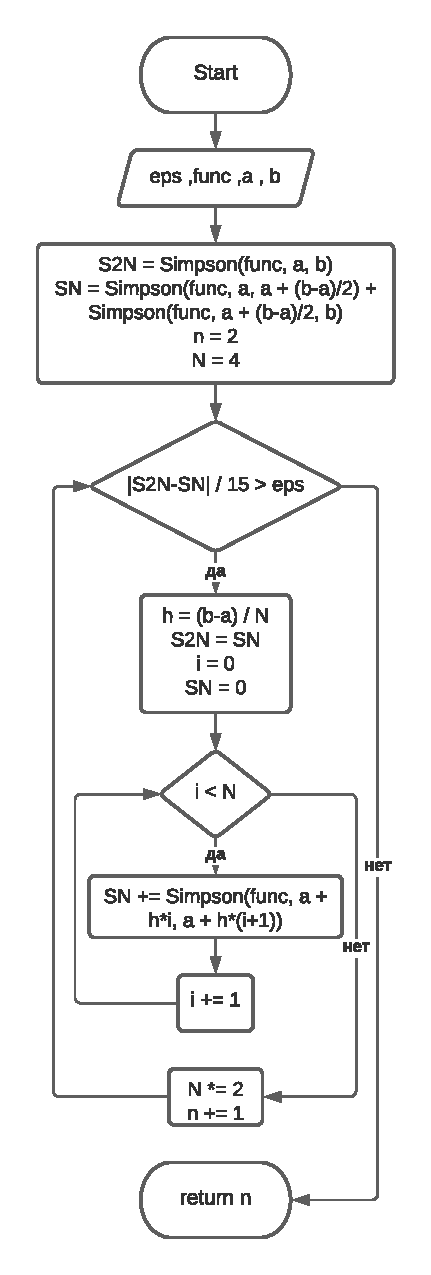
\includegraphics[scale=0.9]{block3.pdf}

def epsilon(numberiter ,func ,a , b):

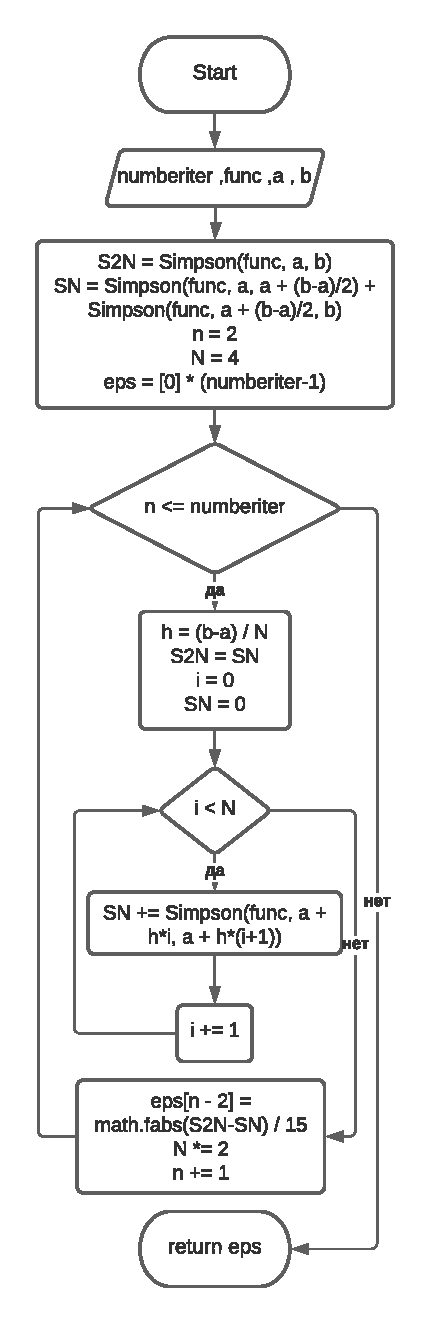
\includegraphics[scale=0.85]{block4.pdf}

def my\_func(x):

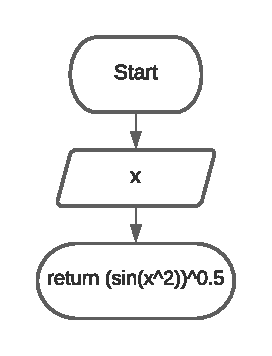
\includegraphics[scale=0.75]{block1.pdf}

def Simpson (func, a, b):

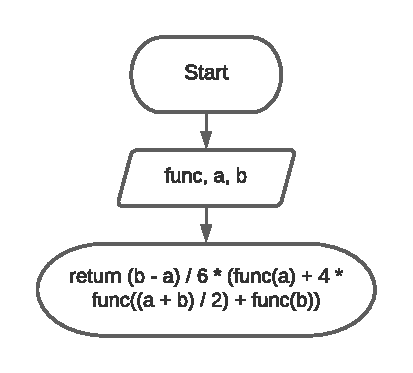
\includegraphics[scale=0.75]{block2.pdf}


\section{Численный анализ решения задачи}


\subsection{Зависимость количества итераций от заданной точности}

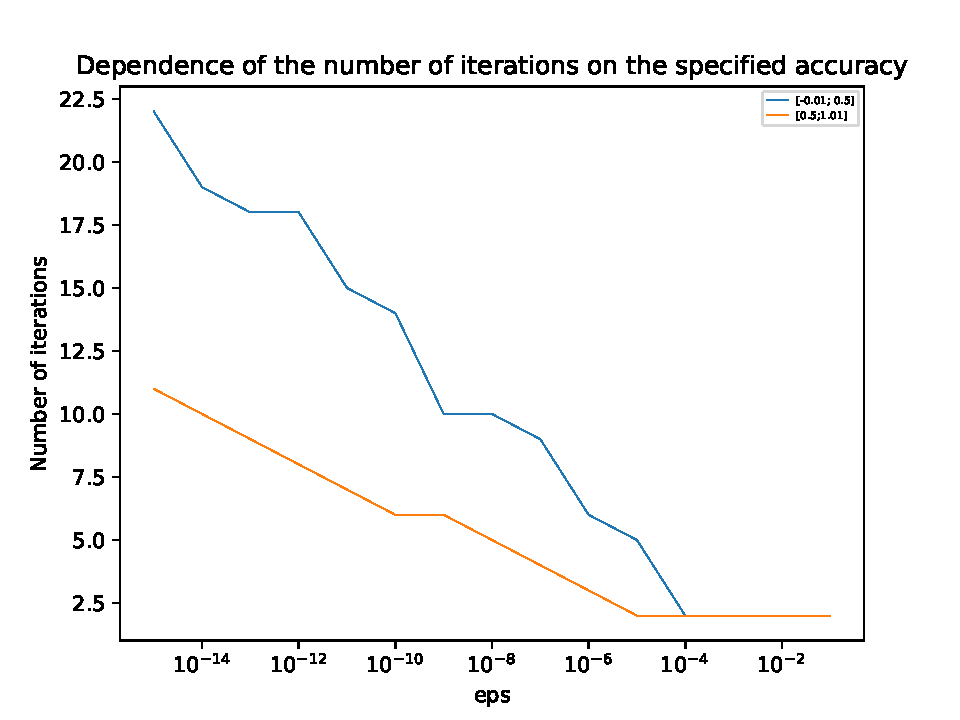
\includegraphics[scale=0.75]{1.pdf}

Как видно из данного графика, для достижения наибольшей точности нужно проделать больше итераций. Для отрезка с разрывом функции это количество существенно больше, чем для отрезка, где функция гладкая. При небольшой точности график выходит на плато. Это обусловлено тем, что значение, вычисляемое при первой итерации имеет точность примерно 10е-4.

\subsection{Сходимость метода}

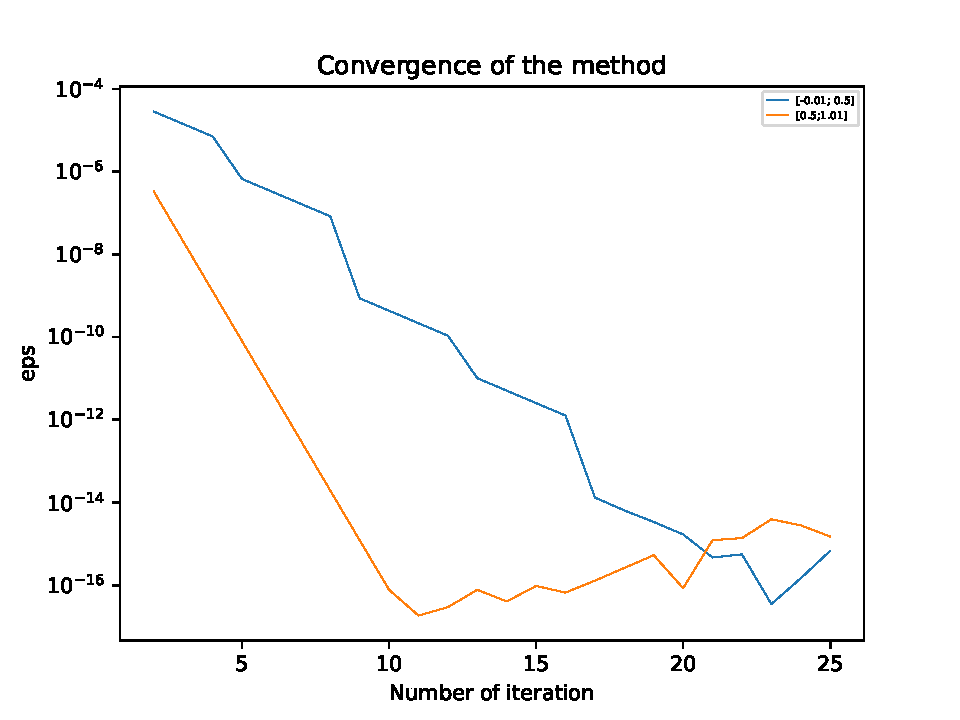
\includegraphics[scale=0.75]{2.pdf}

Как видно из данного графика, при увеличении количества итераций ошибка вычислений уменьшается, но до определнного момента (причем для метода Гаусса с 3 узлами она уменьшается за меньшее количество итераций). Начиная с некоторого количества итераций, ошибка вычислений начинает возрастать для обоих методов. Это обусловлено тем, что при больших n накапливается вычислительная ошибка.

Результаты для гладкого участка функции лучше для обоих методов, чем для участка с разрывом производной.

\section{Краткие выводы}

На основе полученных результатов можно сделать вывод о том, при увеличении количества разбиений для метода Симпсона ошибка вычислений уменьшается, но при больших N накапливается вычислительная ошибка, что приводит к тому, что ошибка результата начинает увеличиваться. Следовательно с помощью обобщенной формулы Симпсона можно достичь лишь некоторой точности (примерно 10е-16 для заданной функции),после чего увеличение количества итераций ухудшает результат. Для гладких участков функции необходимой точности можно достичь за меньшее количество итераций, чем для участков с разрывом производной.

\end{document}
